\section{System Architecture and Core Components}
\noindent

\subsection{System Architecture Overview}

Figure~\ref{fig:Figure_4.1.png} illustrates the overall architecture of the proposed Modbus anomaly detection system in a virtualized testbed environment. The system consists of three layers: the attack simulation layer, the OT simulation layer, and the security monitoring layer. The attack layer uses Kali Linux, Nmap, and Python scripts to generate Modbus probing and malicious traffic, which is transmitted through the vSwitch to ModbusPal in the OT layer.

ModbusPal acts as a PLC simulator and produces register values or exception codes in response to Modbus TCP requests. Meanwhile, Suricata IDS passively monitors the request-response traffic through the virtual network interface and performs packet capture and DPI. The generated eve.json event logs are forwarded to Graylog SIEM for correlation analysis, alert notification, dashboard visualization, and storage.

\begin{figure}[htbp]
\centering
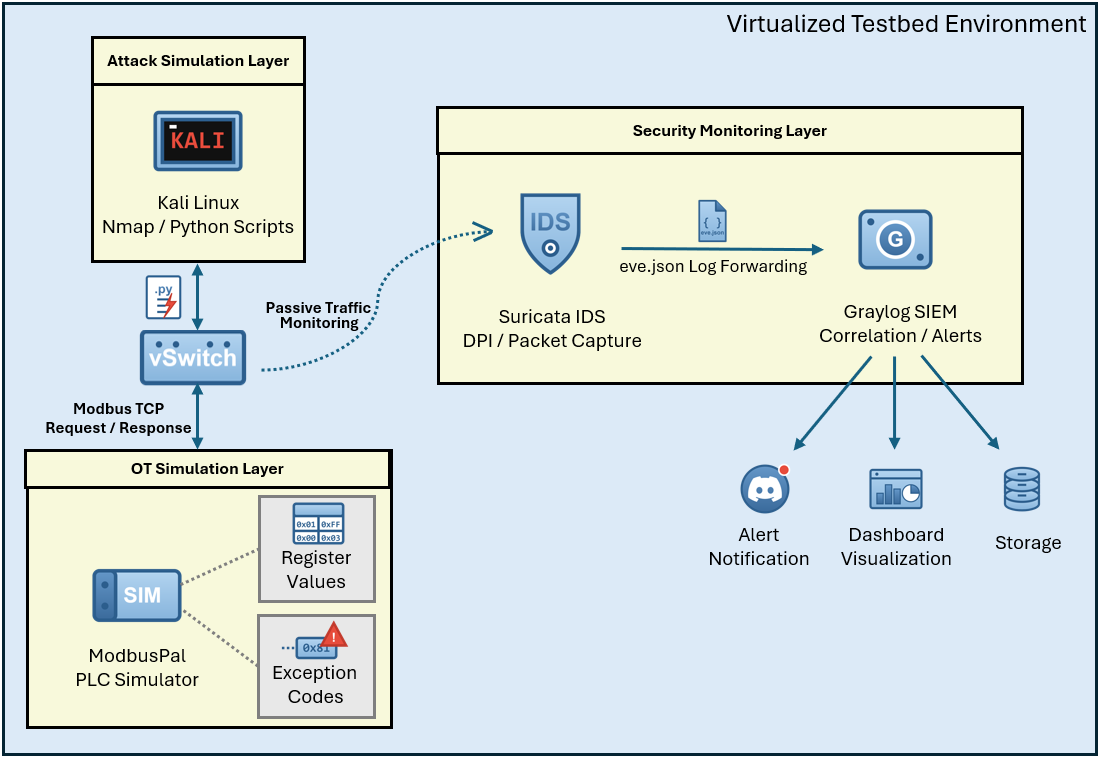
\includegraphics[width=14.5cm]{figure/Figure_4.1.png}
\caption{Overall architecture of the proposed Modbus anomaly detection system in a virtualized testbed environment} \label{fig:Figure_4.1.png}
\end{figure}

\newpage

\subsection{Logical Layer and Component Design}
To ensure that attack validation and security monitoring can be conducted without acting as an inline gateway or modifying the communication path in the testbed, the virtualized testbed is divided into three independent layers:

\begin{itemize}
    \item \textbf{Attack Simulation Layer:} This layer is deployed in an independent virtual machine to simulate threats originating from external networks. Kali Linux is used as the attack platform, while Nmap is used for reconnaissance scanning. In addition, automated Python scripts are used to generate malformed Modbus packets and unauthorized command requests.

    \item \textbf{OT Simulation Layer:} This layer adopts the Java-based ModbusPal \cite{ref_report31} as the PLC simulator to establish a stable industrial communication baseline. Depending on the received Modbus TCP requests, the simulator returns register values or exception codes, thereby emulating the behavior of an operational OT device.

    \item \textbf{Security Monitoring Layer:} This layer serves as the defensive core of the system. In the experimental implementation, this layer may be deployed on the same virtual machine as the OT simulation layer while remaining logically separated by function.Suricata IDS passively monitors the Modbus TCP request-response traffic through the virtual network interface and performs deep packet inspection and signature-based detection. The generated eve.json event logs are then forwarded to Graylog SIEM for visualization, alert generation, log storage, and correlation analysis.
\end{itemize}
\newpage
\section{DPI and SIEM Design}
To achieve the proposed security objectives and standards alignment, this study organizes the monitoring framework as a continuous closed-loop data-processing pipeline. Rather than functioning as isolated detection components, the deep packet inspection (DPI) and security information and event management (SIEM) layers are tightly integrated to transform raw network traffic into alerts with contextual information.

Figure~\ref{fig:Figure_4.0.png} presents the end-to-end processing pipeline, which consists of four systematic operational stages:

\begin{figure}[htbp]
\centering
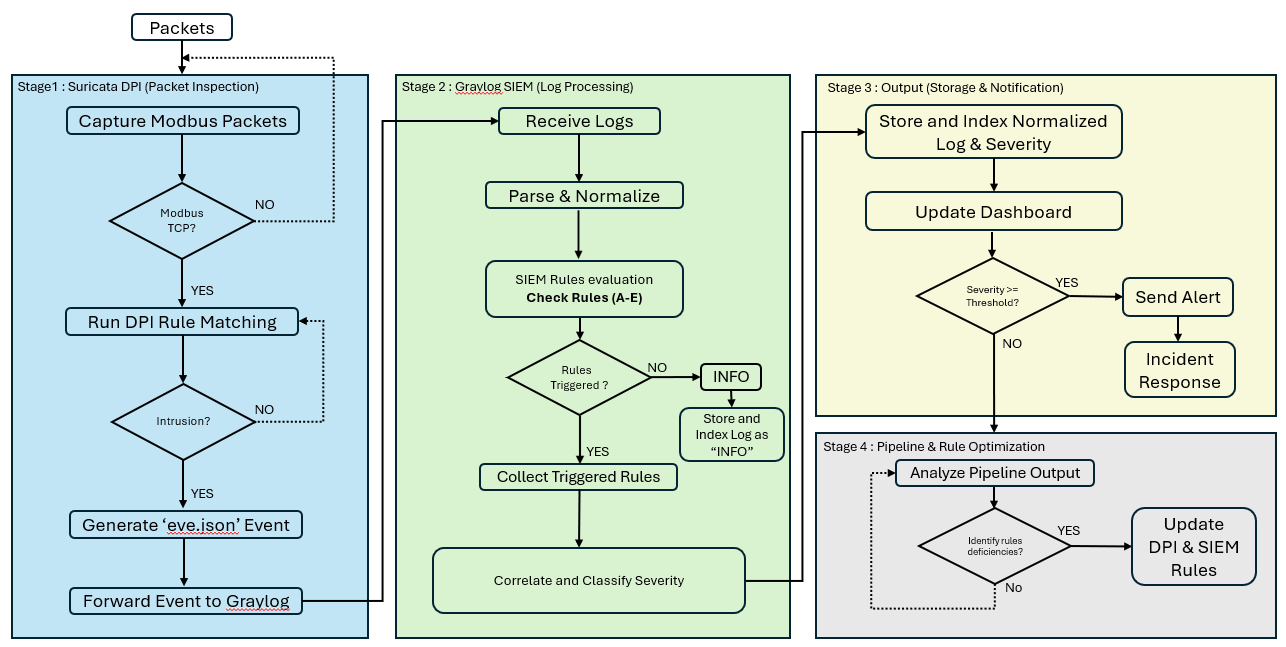
\includegraphics[width=14.5cm]{figure/Figure_4.0.png}
\caption{System Core Processing} \label{fig:Figure_4.0.png}
\end{figure}

\begin{enumerate}
    \newpage
    \item \textbf{Stage 1: Suricata DPI (Packet Inspection):} The pipeline begins at the network interface layer, where Suricata passively captures Modbus TCP traffic in transit. A packet-level parser first performs structural validation to identify Modbus traffic and filter malformed frames. Packets that conform to protocol specifications are then subjected to deep packet inspection using the proposed signature ruleset (e.g., advanced keywords such as \texttt{byte\_test}), producing detailed anomaly events in structured JSON format (\texttt{eve.json}).
    \item \textbf{Stage 2: Graylog SIEM (Log Processing \& Normalization):} After receiving the JSON logs, the SIEM layer ingests, parses, and normalizes the raw values into standardized indexed fields, such as IP addresses, function codes, and payload values. The correlation engine then evaluates these normalized events against scenario-based rules (Scenarios A through E) within predefined temporal windows, dynamically assigning severity and confidence levels.

    \item \textbf{Stage 3: Output (Storage \& Notification):} The processed security events are indexed into the search database to update the operational dashboards in real time. Importantly, when an event is classified as high severity, such as unauthorized register modification or denial-of-service flooding, an automated webhook immediately triggers a Slack notification, enabling maintenance personnel to respond within seconds.

    \item \textbf{Stage 4: Feedback \& Continuous Optimization Loop:} To mitigate alert fatigue and accommodate site-specific environments, the framework incorporates a continuous feedback loop. Security analysts review pipeline outputs and audit trails of both triggered and untriggered events to identify rule deficiencies, thereby enabling periodic and fine-grained refinement of both the Suricata DPI rules and the Graylog correlation thresholds.
\end{enumerate}

\noindent
\subsection{Protocol Parsing and Security Pre-check}
Figure~\ref{fig:Figure_4.2.png} illustrates the Modbus TCP protocol parsing, security pre-check, and rule-based deep packet inspection workflow. The proposed inspection logic is developed based on the deep packet inspection approach described in Al-Dalky et al. \cite{ref_report18}. In this process, the system first parses the MBAP header and extracts the Protocol ID, Length, and Unit ID fields for validation to determine whether the received packet conforms to the expected Modbus TCP format. This security pre-check is used to identify malformed or structurally invalid packets before deeper inspection is performed. If a packet fails the pre-check, it is classified as suspicious traffic and logged for further analysis. If the packet passes validation, the system proceeds to the DPI stage, where function code analysis, payload inspection, and rule-based detection are performed. This two-stage design ensures that the downstream detection process operates on well-formed traffic and reduces unnecessary noise. 

\begin{figure}[htbp]
\centering
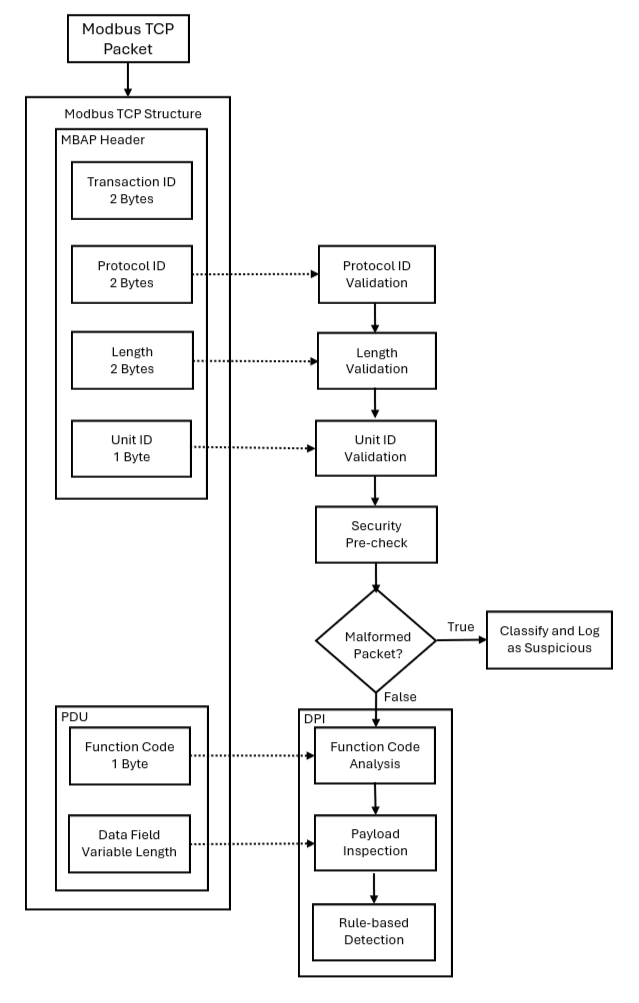
\includegraphics[width=14.5cm]{figure/Figure_4.2.png}
\caption{Overall architecture of the proposed Modbus anomaly detection system in a virtualized testbed environment} \label{fig:Figure_4.2.png}
\end{figure}

\newpage

\subsection{Modbus Function Code and Exception Response Detection Logic}
Modbus TCP communication mainly relies on Function Codes to indicate the operation requested by the client, such as reading Coils, reading Holding Registers, or writing control parameters. Therefore, Function Codes provide a direct basis for identifying the intent of a Modbus TCP request. In this research, request-side Function Codes are inspected to detect read operations, write operations, diagnostic access, management-related functions, and unsupported Function Codes.

Since write operations can directly modify Coils or Holding Registers, they are considered more sensitive than read operations. In addition, diagnostic and management-related Function Codes may be used for device testing, identification, or protocol probing. The Function Code detection rules used in this research are summarized in Table \ref{tab:modbus_rules_final}.
\begin{table}[htbp]
\caption{Modbus Function Code Rules and Security Implications}
\centering
\resizebox{\textwidth}{!}{%
\begin{tabular}{|>{\centering\arraybackslash}m{2.6cm}|>{\centering\arraybackslash}m{2.0cm}|>{\centering\arraybackslash}m{2.8cm}|m{4.2cm}|m{4.8cm}|}
\hline
\textbf{Type} & \textbf{Code / Cond.} & \textbf{Name} & \textbf{Logic} & \textbf{Security Implication} \\ \hline

MBAP Header Check & ID $\neq$ 0x0000 & Abnormal Protocol Identifier & Check whether the Protocol Identifier in the MBAP Header is not 0x0000. & May indicate malformed Modbus TCP packets or non-standard traffic. \\ \hline

Read FC & FC01 / 0x01 & Read Coils & Detect Function Code 0x01 in the request PDU. & Large volumes or unauthorized sources may indicate reconnaissance. \\ \hline

Read FC & FC02 / 0x02 & Read Discrete Inputs & Detect Function Code 0x02 in the request PDU. & May indicate digital input status collection. \\ \hline

Read FC & FC03 / 0x03 & Read Holding Registers & Detect Function Code 0x03 in the request PDU. & May expose control parameters or process values. \\ \hline

Read FC & FC04 / 0x04 & Read Input Registers & Detect Function Code 0x04 in the request PDU. & May indicate sensor or process data collection. \\ \hline

Write FC & FC05 / 0x05 & Write Single Coil & Detect Function Code 0x05 in the request PDU. & May directly change device states. \\ \hline

Write FC & FC06 / 0x06 & Write Single Register & Detect Function Code 0x06 in the request PDU. & May modify control parameters or setpoints. \\ \hline

Diagnostic FC & FC08 / 0x08 & Diagnostics & Detect Function Code 0x08 in the request PDU. & May indicate diagnostic access or protocol probing. \\ \hline

Write FC & FC15 / 0x0F & Write Multiple Coils & Detect Function Code 0x0F in the request PDU. & May change multiple device states at once. \\ \hline

Write FC & FC16 / 0x10 & Write Multiple Registers & Detect Function Code 0x10 in the request PDU. & May modify multiple process parameters. \\ \hline

Identification FC & FC17 / 0x11 & Report Server ID & Detect Function Code 0x11 in the request PDU. & May expose device identity or server information and can be used for device enumeration. \\ \hline

Advanced Write FC & FC22 / 0x16 & Mask Write Register & Detect Function Code 0x16 in the request PDU. & May alter selected bits of a register. \\ \hline

Mixed R/W FC & FC23 / 0x17 & Read/Write Multiple Registers & Detect Function Code 0x17 in the request PDU. & Combines data collection and value modification. \\ \hline

Management FC & FC43 / 0x2B & Encapsulated Interface Transport & Detect Function Code 0x2B in the request PDU. & May expose device identity, vendor information, or management-related information. \\ \hline

Unsupported FC & Not in allowed FC list & Unsupported Function Code & Detect Function Codes outside the allowed operation set. & May indicate probing, fuzzing, or malformed requests. \\ \hline

\end{tabular}%
}
\label{tab:modbus_rules_final}
\end{table}
\newpage
When a Server or PLC cannot process a client request normally, it returns an
Exception Response to indicate that the request contains an abnormal
function, address, data value, or device condition. In a normal response,
the server replies with the same Function Code as the original request.
If an exception occurs, the server sets the most significant bit of the
original Function Code to 1. In other words, the response Function Code
equals the original Function Code plus \texttt{0x80}:

$$
\mathrm{ExceptionFunctionCode} = \mathrm{OriginalFunctionCode} + \texttt{0x80}
$$

It can also be checked using the following bitwise condition:

$$
\mathrm{FunctionCode} \ \&\ \texttt{0x80} = \texttt{0x80}
$$

For example, if a client sends Function Code \texttt{0x03} to read Holding
Registers but the requested address is invalid, the server may return
Function Code \texttt{0x83} with Exception Code \texttt{0x02}, which
represents \emph{Illegal Data Address}. Similarly, if an FC17 /
\texttt{0x11} Report Server ID request fails, the response Function Code
becomes \texttt{0x91}, followed by the corresponding Exception Code.

Exception Responses are important anomaly indicators in Modbus TCP traffic. A single Exception Response does not necessarily indicate an attack, as it may also result from misconfiguration, an inconsistent address map, or operational mistakes. However, if Exception Responses appear frequently within a short period, or occur together with unsupported Function Codes, abnormal MBAP Headers, or scanning behavior, they may indicate protocol probing, fuzzing, or device capability enumeration.

In this research, Modbus Exception Codes are included in the detection rules and SIEM correlation analysis to support the identification of abnormal requests and potential attack behaviors. The Exception Response detection rules are shown in Table \ref{tab:modbus_exception_rules}.
\begin{table}[htbp]
\caption{Modbus Exception Code Rules and Security Implications}
\centering
\resizebox{\textwidth}{!}{%
\begin{tabular}{|>{\centering\arraybackslash}m{2.0cm}|>{\centering\arraybackslash}m{4.0cm}|m{5.0cm}|m{5.2cm}|}
\hline
\textbf{Exception Code} & \textbf{Exception Name} & \textbf{Detection Logic} & \textbf{Security Implication} \\ \hline

\texttt{0x01} & Illegal Function & Detect response Function Code with \texttt{0x80} flag and Exception Code \texttt{0x01}. & May indicate unsupported Function Code probing or fuzzing. \\ \hline

\texttt{0x02} & Illegal Data Address & Detect response Function Code with \texttt{0x80} flag and Exception Code \texttt{0x02}. & May indicate address enumeration or unauthorized address access. \\ \hline

\texttt{0x03} & Illegal Data Value & Detect response Function Code with \texttt{0x80} flag and Exception Code \texttt{0x03}. & May indicate invalid write values or abnormal request parameters. \\ \hline

\texttt{0x04} & Slave Device Failure & Detect response Function Code with \texttt{0x80} flag and Exception Code \texttt{0x04}. & May indicate device processing failure. \\ \hline

\texttt{0x05} & Acknowledge & Detect response Function Code with \texttt{0x80} flag and Exception Code \texttt{0x05}. & Indicates that the request requires longer processing time. \\ \hline

\texttt{0x06} & Slave Device Busy & Detect response Function Code with \texttt{0x80} flag and Exception Code \texttt{0x06}. & May indicate device busy state or excessive requests. \\ \hline

\texttt{0x07} & Negative Acknowledge & Detect response Function Code with \texttt{0x80} flag and Exception Code \texttt{0x07}. & May indicate rejected diagnostic or programming requests. \\ \hline

\texttt{0x08} & Memory Parity Error & Detect response Function Code with \texttt{0x80} flag and Exception Code \texttt{0x08}. & May indicate memory, hardware, or integrity-related errors. \\ \hline

\texttt{0x0A} & Gateway Path Unavailable & Detect response Function Code with \texttt{0x80} flag and Exception Code \texttt{0x0A}. & May indicate gateway or downstream routing issues. \\ \hline

\texttt{0x0B} & Gateway Target Device Failed to Respond & Detect response Function Code with \texttt{0x80} flag and Exception Code \texttt{0x0B}. & May indicate downstream device failure, network interruption, or service unavailability. \\ \hline

\end{tabular}%
}
\label{tab:modbus_exception_rules}
\end{table}
\newpage
Overall, this research combines request-side Function Code inspection with response-side Exception Response detection. This design allows the system to identify both high-risk client operations and abnormal server responses, providing a more complete basis for SIEM correlation analysis and Modbus TCP anomaly detection.

\subsection{SIEM Log Ingestion and Correlation Design}
Figure~\ref{fig:Figure_4.3.png} illustrates the log forwarding and SIEM correlation workflow between Suricata and Graylog. After Modbus TCP packets are inspected by Suricata through packet-level rule matching, the generated eve.json events are forwarded to Graylog for centralized log processing. Graylog then performs log reception, parsing and normalization, SIEM rule triggering, and correlation-based severity classification. The processed events are subsequently stored and indexed, visualized through dashboards, and delivered through alert notification mechanisms.
This SIEM-layer design is particularly important for threshold-based detection scenarios, such as DoS flooding, where Graylog evaluates the number of matched events within a defined time window before triggering an alert.

\begin{figure}[htbp]
\centering
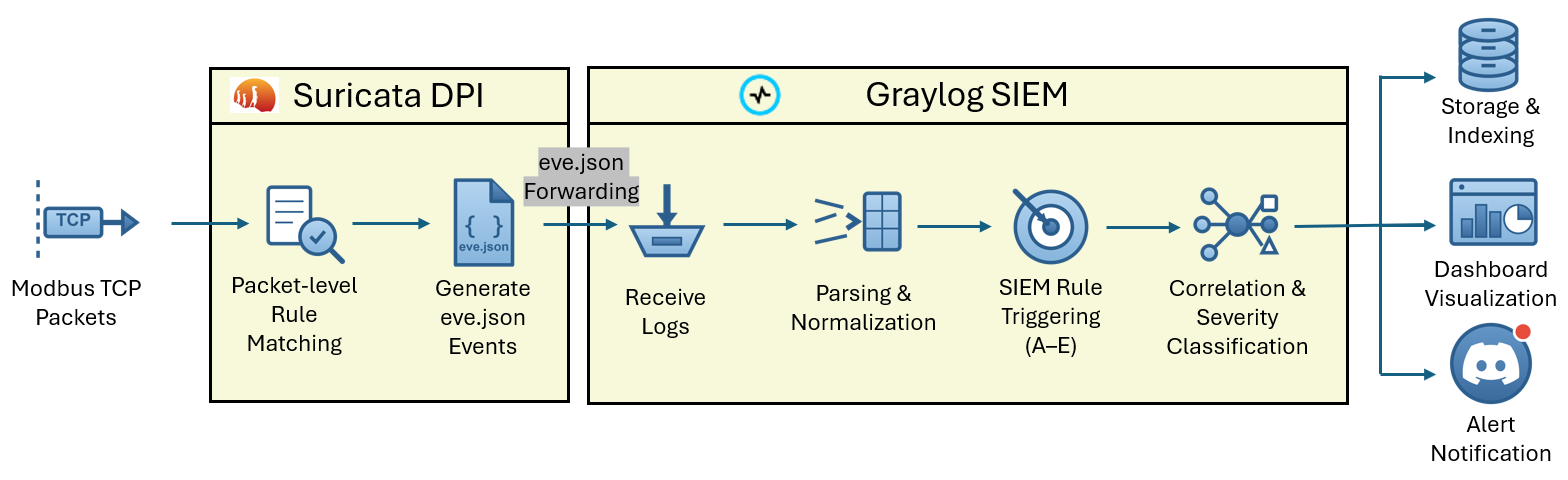
\includegraphics[width=13.5cm]{figure/Figure_4.3.png}
\caption{Suricata-to-Graylog SIEM Log Processing and Correlation Workflow} \label{fig:Figure_4.3.png}
\end{figure}

\newpage

\section{Scenario-based Detection Rule Design}
This research proposes scenario-based detection rules derived from representative Modbus TCP attack behaviors. The proposed rules are mapped to ICS Cyber Kill Chain Stage 2, ISA/IEC 62443-3-3 foundational requirements, and MITRE ATT\&CK for ICS techniques. Suricata is used to detect packet-level and application-layer features, while Graylog aggregates events, evaluates contextual conditions, assigns priorities, and generates alerts.

The detection scenarios cover reconnaissance, request-side protocol probing, response-side exception detection, unauthorized write operations, advanced register manipulation, diagnostic command injection, and denial-of-service activities at both the connection and application layers. For each scenario, the objective, traffic direction, key traffic characteristics, detection basis, and expected alert behavior are defined before the corresponding Suricata rules and Graylog correlation logic are presented. Table~\ref{tab:detection_tool_mapping} summarizes the proposed detection scenarios and their detection focus.
\begin{table}[htbp]
\caption{Detection Scenarios, Evidence, and Corresponding Testing Tools}
\centering
\footnotesize
\renewcommand{\arraystretch}{1.5}

\resizebox{\textwidth}{!}{%
\begin{tabular}{|>{\bfseries\centering\arraybackslash}m{1.3cm}
                |>{\centering\arraybackslash}m{3.8cm}
                |>{\centering\arraybackslash}m{5.0cm}
                |>{\centering\arraybackslash}m{3.0cm}|}
\hline
\textbf{Scenario} & 
\textbf{Detection Scenario} & 
\textbf{Main Detection Evidence} & 
\textbf{Tool / Method} \\ 
\hline

A 
& Reconnaissance Scanning 
& TCP/502 access and Modbus service discovery behavior 
& Nmap modbus-discover \\ 
\hline

B1 
& Request-side Modbus Protocol Probing 
& Sensitive, uncommon, or unsupported Function Codes 
& Python socket script \\ 
\hline

B2 
& Response-side Modbus Exception 
& Exception Function Code with \texttt{0x80} flag and Exception Code 
& Python socket script \\ 
\hline

C1 
& Unauthorized Modification 
& FC05 / FC06 write requests from non-whitelisted sources 
& pymodbus \\ 
\hline

C2 
& Advanced Register Manipulation 
& FC22 / FC23 advanced register operations 
& pymodbus \\ 
\hline

D 
& Critical Diagnostic Command Injection 
& FC08 diagnostic command pattern 
& Python socket script \\ 
\hline

E1 
& Modbus TCP/502 High-rate SYN Activity 
& Excessive TCP SYN packets 
& hping3 SYN flood \\ 
\hline

E2 
& Modbus TCP/502 High-rate Payload Activity 
& Excessive Modbus TCP payload-bearing requests 
& Python socket script \\ 
\hline

\end{tabular}%
}
\label{tab:detection_tool_mapping}
\end{table}

\subsection{Scenario A - Reconnaissance Scanning}During the test stage, Scenario A detects reconnaissance scanning through FC17 Report Server ID and FC43 Read Device Identification, which may reveal device identity, operational status, and hardware, firmware, or product information. Although these functions do not directly alter device states, their use from unauthorized sources or at abnormal times may indicate target profiling before an attack. This scenario maps to the Test stage of ICS Cyber Kill Chain Stage 2, FR 5 Restricted Data Flow in ISA/IEC 62443-3-3, and T0846 Remote System Discovery in MITRE ATT\&CK for ICS.

\subsection{Scenario B1 - Request-side Modbus Protocol Probing}Scenario B1 detects abnormal Modbus requests in the client-to-server direction, focusing on unsupported Function Codes and invalid MBAP Protocol Identifiers. In Modbus TCP, the MBAP Protocol Identifier should normally be 0x0000; a non-zero value may indicate a malformed packet or protocol probing attempt. Requests using unusual or unsupported Function Codes may also suggest fuzzing or attempts to identify supported device functions and parsing weaknesses. This scenario maps to the Deliver stage of ICS Cyber Kill Chain Stage 2, FR 3 System Integrity in ISA/IEC 62443-3-3, and T0846 Remote System Discovery in MITRE ATT\&CK for ICS.

\subsection{Scenario B2 - Response-side Modbus Exception }Scenario B2 detects Modbus Exception Responses in the server-to-client direction. When a PLC or Modbus server cannot process a request, the response Function Code is set to the original Function Code plus 0x80, followed by an Exception Code indicating the error cause, such as Illegal Function, Illegal Data Address, or Illegal Data Value. While Exception Responses are not necessarily malicious, frequent occurrences or correlation with unsupported Function Codes, illegal address access, or scanning behavior may indicate protocol probing, device enumeration, or fuzzing. This scenario maps to the Deliver stage of ICS Cyber Kill Chain Stage 2, FR 3 System Integrity in ISA/IEC 62443-3-3, and T0846 Remote System Discovery in MITRE ATT\&CK for ICS.

\subsection{Scenario C1 - Unauthorized Modification}Scenario C1 detects Modbus write commands from unauthorized sources, including FC05 Write Single Coil, FC06 Write Single Register, FC15 Write Multiple Coils, and FC16 Write Multiple Registers. Since these functions can directly modify coil states or holding register values, unauthorized use may cause process parameter changes, abnormal control states, or device misoperation. Suricata identifies write-related Function Codes, while Graylog correlates them with source IP addresses, asset roles, and whitelist conditions to determine whether the operation is authorized. This scenario maps to the Install / Modify stage of ICS Cyber Kill Chain Stage 2, FR 2 Use Control in ISA/IEC 62443-3-3, and T0836 Modify Parameter in MITRE ATT\&CK for ICS.

\subsection{Scenario C2 - Advanced Register Manipulation}Scenario C2 detects advanced Modbus register operations, including FC22 Mask Write Register and FC23 Read/Write Multiple Registers. Compared with general write commands, FC22 can modify specific bits of a holding register, while FC23 can read and write multiple registers in a single transaction. These operations provide more precise control over process parameters or control logic and should be treated as high risk when issued by non-whitelisted hosts, outside normal operating periods, or after probing events. This scenario maps to the Install / Modify stage of ICS Cyber Kill Chain Stage 2, FR 3 System Integrity in ISA/IEC 62443-3-3, and T0831 Manipulation of Control in MITRE ATT\&CK for ICS.

\subsection{Scenario D - Critical Diagnostic Command Injection}Scenario D detects Modbus FC08 Diagnostic commands and high-risk sub-functions, including 0x0001 Restart Communications Option, 0x0004 Force Listen Only Mode, and 0x000A Clear Counters and Diagnostic Register. Although FC08 is intended for diagnostics and communication testing, these sub-functions may reinitialize communication, force a device into listen-only mode, or clear diagnostic counters, thereby affecting control communication and incident traceability. When issued from unauthorized sources or outside maintenance windows, such commands should be treated as high-risk behavior. This scenario maps to the Execute ICS Attack stage of ICS Cyber Kill Chain Stage 2, FR 3 System Integrity in ISA/IEC 62443-3-3, and T0816 Device Restart/Shutdown in MITRE ATT\&CK for ICS.

\subsection{Scenario E1 - Modbus TCP/502 High-rate SYN Activity}Scenario E1 detects high-rate TCP SYN activity targeting Modbus TCP port 502. A large number of SYN packets may consume connection-handling capacity, network bandwidth, or controller communication resources, resulting in Modbus service delay or disruption. Suricata uses threshold conditions to count SYN packets from the same source within a short time window and triggers a DoS alert when the count exceeds the configured threshold. This scenario maps to the Execute ICS Attack stage of ICS Cyber Kill Chain Stage 2, FR 7 Resource Availability in ISA/IEC 62443-3-3, and T0814 Denial of Service in MITRE ATT\&CK for ICS.

\subsection{Scenario E2 - Modbus TCP/502 High-rate Payload Activity}Scenario E2 detects high-rate payload-bearing traffic targeting Modbus TCP port 502. Unlike SYN-based detection, this scenario focuses on established connections carrying Modbus payloads, which may force PLCs or Modbus servers to continuously process application-layer requests and create pressure on CPU, memory, or protocol-processing resources. Suricata monitors TCP/502 packets with dsize greater than zero and applies threshold conditions to identify abnormal request rates. This scenario maps to the Execute ICS Attack stage of ICS Cyber Kill Chain Stage 2, FR 7 Resource Availability in ISA/IEC 62443-3-3, and T0814 Denial of Service in MITRE ATT\&CK for ICS.
\newpage

\section{Traceability Matrix and Alert Severity Strategy}
\noindent

\subsection{Alert Severity Classification Design}
In the alert severity section, we designed it in a flexible way to improve the efficiency of incident response within the Graylog platform. After the alerts are integrated, we classify them into three levels:

\begin{itemize}
    \item 
    \textbf{Low Severity (Operational Baseline):} 
    Assigned to routine operational logs, such as authorized HMI read requests. While not an attack, these events are crucial for establishing a deterministic baseline.
    \item
    \textbf{Normal Severity (Early Kill Chain):} Assigned to anomalous activities in the early stages, including Step 1 and Step 2, such as unauthorized scanning. Detecting these events enables operators to preemptively block attacks before physical impacts occur.
    \item
    \textbf{High Severity (Advanced Kill Chain):} Assigned to activities in the advanced stages, including Steps 3 to 5, involving unauthorized parameter modifications or command injections. Such threats directly affect the security and availability emphasized by ISA/IEC 62443.
\end{itemize}
\newpage
\subsection{Traceability Matrix of Proposed Detection Rules}
Finally, the SIEM platform converts these rules and severity levels into a traceability matrix for user reference. The traceability matrix of the proposed detection rules is shown in Table \ref{tab:traceability_matrix}. This matrix maps each detection target to the corresponding ICS Kill Chain stage, ISA/IEC 62443-3-3 Foundational Requirement, MITRE ATT\&CK for ICS technique, and severity level.

\begin{table}[htbp]
\caption{Traceability Matrix of Proposed Detection Rules}
\centering
\normalsize
\renewcommand{\arraystretch}{1.4}

\resizebox{\textwidth}{!}{%
\begin{tabular}{|>{\bfseries\centering\arraybackslash}m{1.6cm}|>{\centering\arraybackslash}m{4.5cm}|>{\centering\arraybackslash}m{2.3cm}|>{\centering\arraybackslash}m{2.6cm}|>{\centering\arraybackslash}m{3.2cm}|>{\centering\arraybackslash}m{1.5cm}|}
\hline
\textbf{Scenario\newline /Rule} & \textbf{Detection Target} & \textbf{ICS Cyber Kill Chain Stage} \cite{ref_report16} & \textbf{ISA/IEC 62443-3-3} \cite{ref_report15} & \textbf{MITRE ATT\&CK for ICS} \cite{ref_report17} & \textbf{Severity} \\ \hline

A & FC17 Report Server ID and FC43 Read Device Identification & Test & FR 5 - Restrict Data Flow & T0846 - Remote System Discovery & Normal \\ \hline

B1 & Unsupported Function Code and invalid MBAP Protocol ID & Deliver & FR 3 - System Integrity & T0846 - Remote System Discovery & Normal \\ \hline

B2 & Modbus Exception Responses returned by server & Deliver & FR 3 - System Integrity & T0846 - Remote System Discovery & Normal \\ \hline

C1 & FC05, FC06, FC15, and FC16 write operations & Install / Modify & FR 2 - Use Control & T0836 - Modify Parameter & High \\ \hline

C2 & FC22 Mask Write Register and FC23 Read/Write Multiple Registers & Install / Modify & FR 3 - System Integrity & T0831 - Manipulation of Control & High \\ \hline

D & FC08 diagnostic sub-functions, including Restart Communications and Force Listen Only Mode & Execute ICS Attack & FR 3 - System Integrity & T0816 - Device Restart/Shutdown & High \\ \hline

E1 & High-rate SYN packets targeting TCP/502 & Execute ICS Attack & FR 7 - Resource Availability & T0814 - Denial of Service & High \\ \hline

E2 & High-rate payload-bearing Modbus TCP requests & Execute ICS Attack & FR 7 - Resource Availability & T0814 - Denial of Service & High \\ \hline

\end{tabular}%
}
\label{tab:traceability_matrix}
\end{table}


\newpage
